\newpage
\section{Thiết kế hệ thống qua lược đồ (System Design Diagrams)}

Để cụ thể hóa cấu trúc và luồng xử lý của 8 Use-case trên, chương này trình bày các lược đồ thiết kế hệ thống theo tiêu chuẩn UML.

\subsection{Lược đồ Use-case tổng quát}
Lược đồ Use-case mô tả mối quan hệ giữa các tác nhân và các chức năng của hệ thống, phân định rõ ràng giữa nhiệm vụ của Task 1 và Task 2.

\begin{figure}[H]
    \centering
    \includegraphics[width=0.9\textwidth]{image/usecase_general.png}
    \caption{Sơ đồ Use-case tổng quát của hệ thống Website doanh nghiệp}
\end{figure}

\subsection{Lược đồ Thực thể Mối quan hệ (ERD)}
Cơ sở dữ liệu được thiết kế theo chuẩn để đảm bảo tính toàn vẹn dữ liệu cho các tính năng quản trị nội dung tĩnh và tiếp nhận thông tin khách hàng.

\begin{figure}[H]
    \centering
    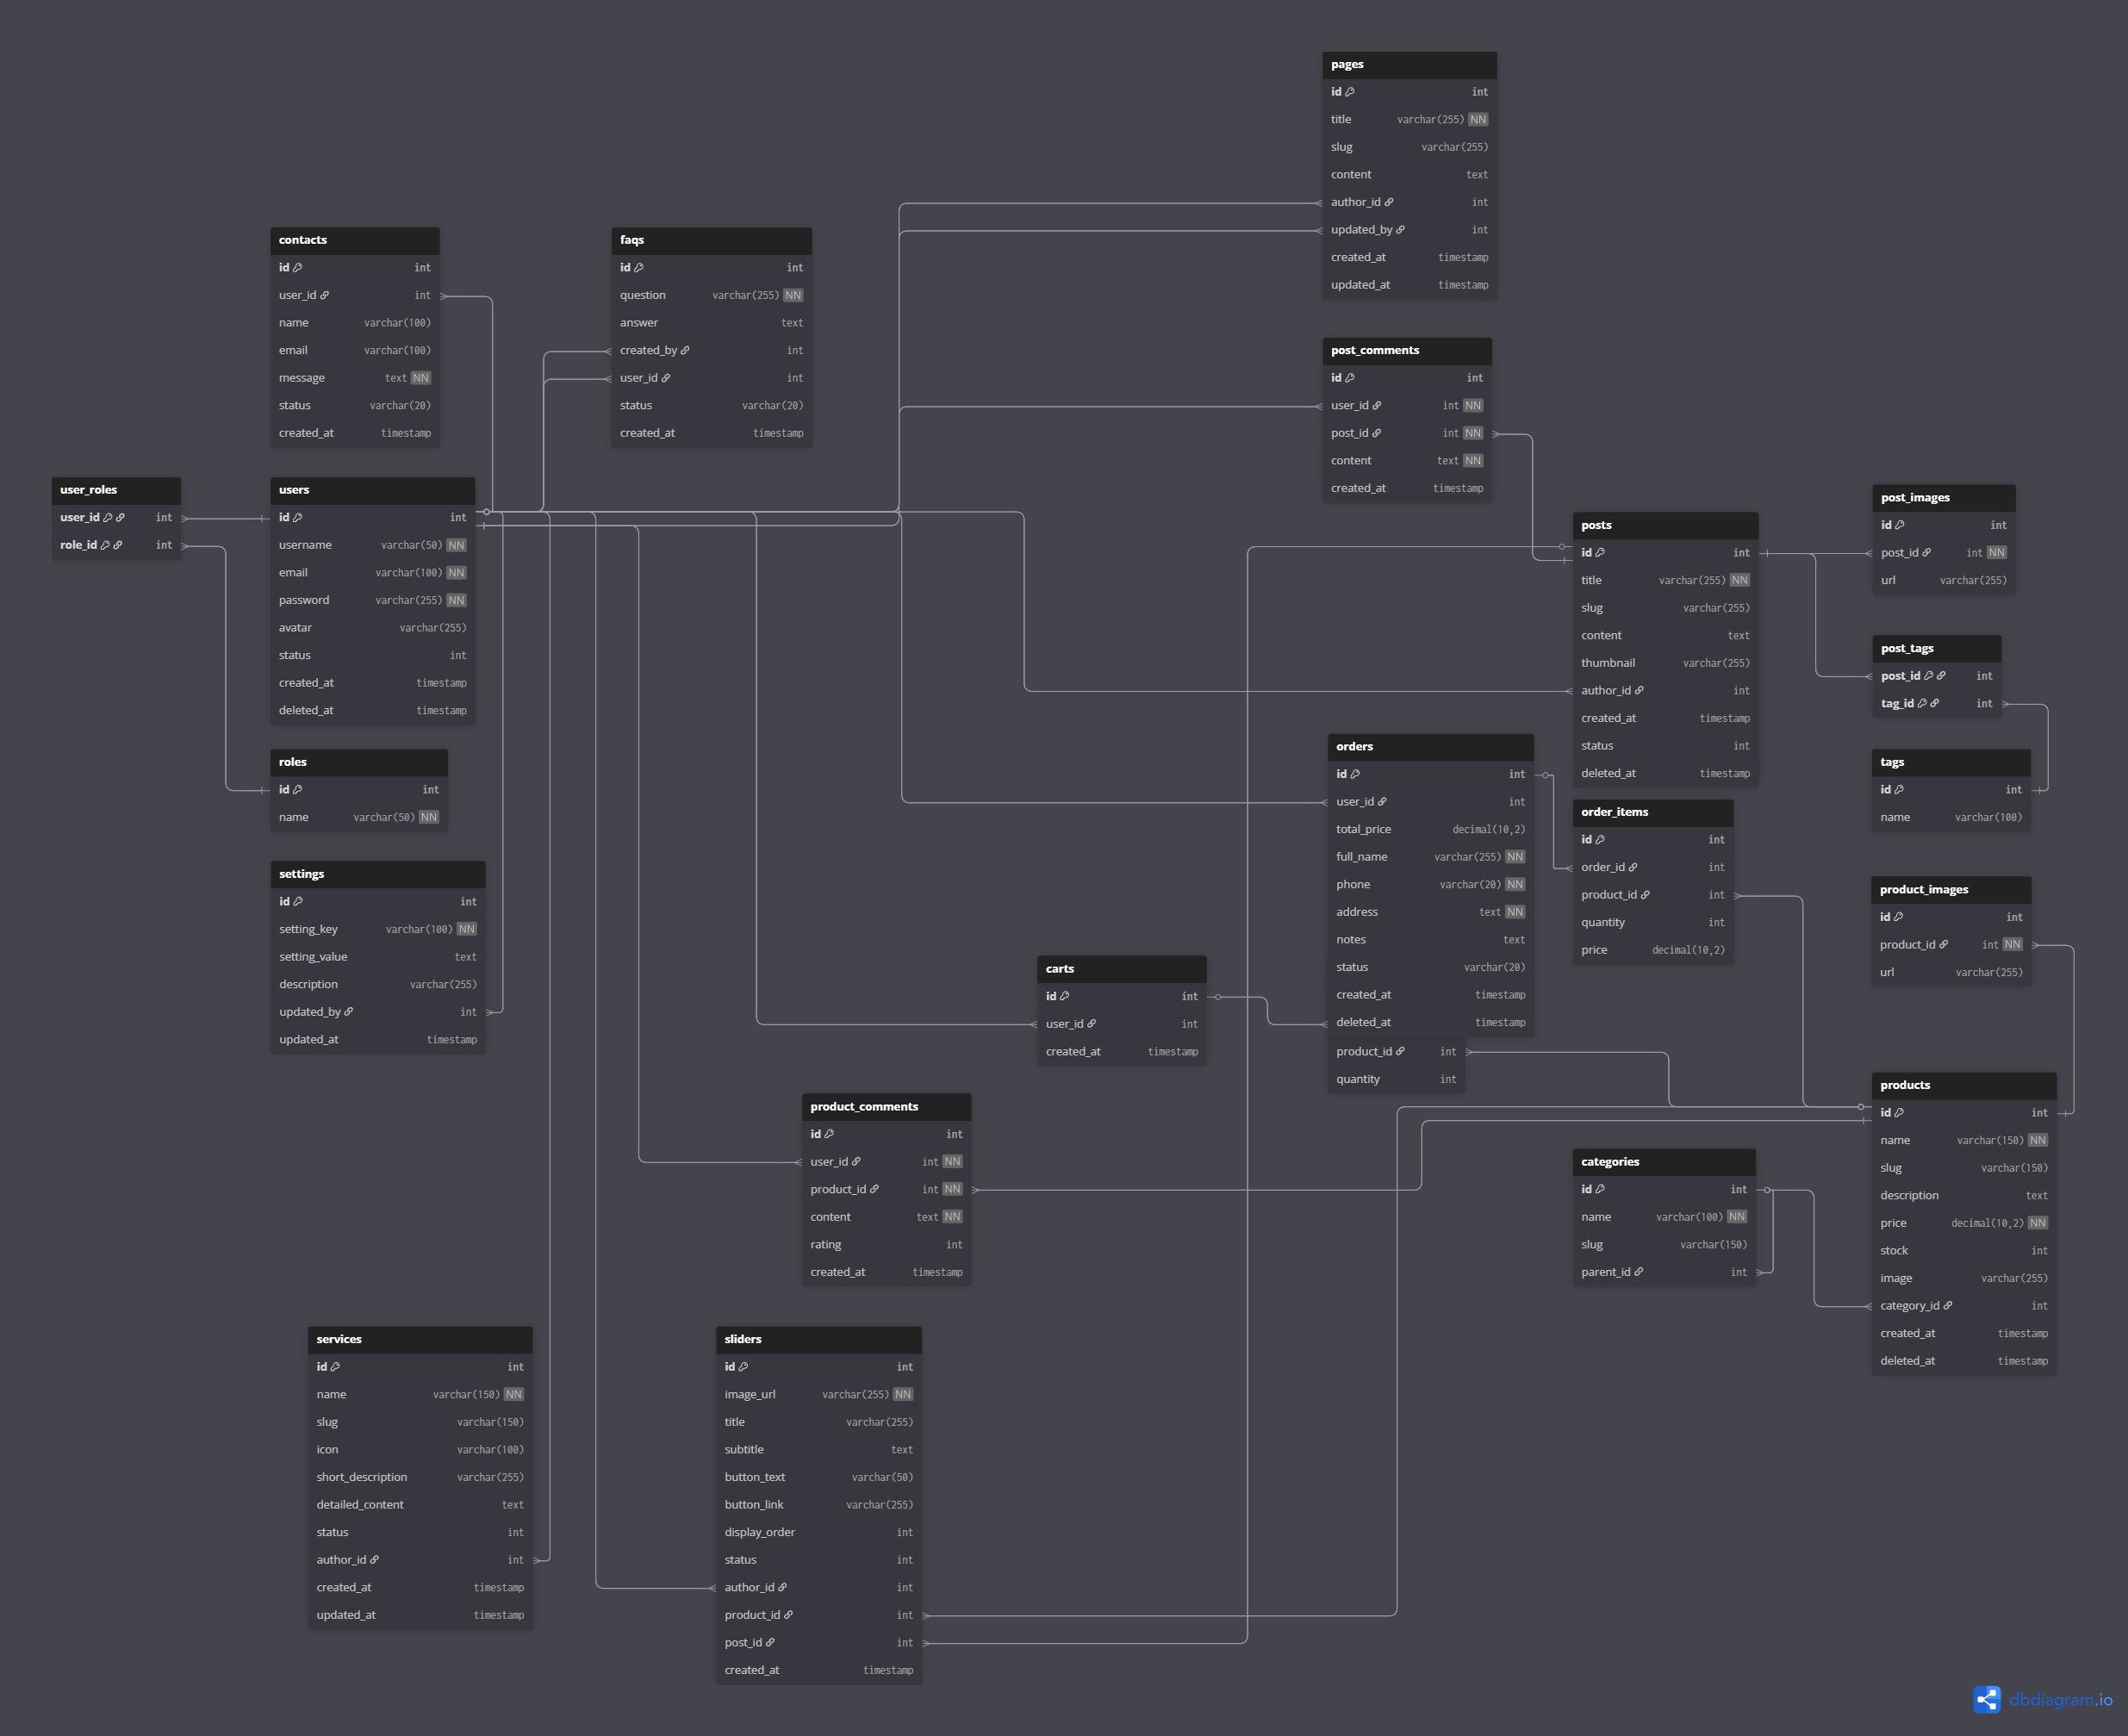
\includegraphics[width=0.85\textwidth]{image/erd_diagram.png}
    \caption{Sơ đồ thực thể mối quan hệ (ERD) cho hệ thống quản trị}
\end{figure}

\subsection{Lược đồ Hoạt động cho chức năng Gửi liên hệ (UC-GUE-001)}
Mô tả chi tiết các bước kiểm tra logic từ phía người dùng (Frontend) đến phía máy chủ (Backend).

\begin{figure}[H]
    \centering
    \includegraphics[width=0.7\textwidth]{image/activity_contact.png}
    \caption{Sơ đồ hoạt động (Activity Diagram) của chức năng Gửi liên hệ}
\end{figure}

\subsection{Lược đồ Trình tự cho chức năng Đăng nhập (UC-ADM-001)}
Minh họa sự tương tác giữa các lớp trong mô hình MVC để thực hiện xác thực quyền quản trị.

\begin{figure}[H]
    \centering
    \includegraphics[width=0.9\textwidth]{image/sequence_login.png}
    \caption{Sơ đồ trình tự (Sequence Diagram) cho quy trình Đăng nhập}
\end{figure}

\subsection{Lược đồ Cấu trúc thư mục mã nguồn (MVC)}
Hệ thống được tổ chức theo mô hình MVC tự viết, tách biệt rõ ràng giữa logic xử lý, giao diện và tương tác dữ liệu.

\begin{figure}[H]
    \centering
    \includegraphics[width=0.6\textwidth]{image/folder_structure.png}
    \caption{Sơ đồ cấu trúc thư mục dự án PHP thuần}
\end{figure}

\newpage
\section{Thiết kế giao diện người dùng (Mockup-UI)}

Dựa trên các kịch bản vận hành đã phân tích, chương này trình bày các bản phác thảo giao diện (Mockup) cho hệ thống Website doanh nghiệp. Giao diện được thiết kế theo mô hình quản trị nội dung (CMS), đảm bảo tính đồng nhất giữa phía người dùng (Frontend) và phía quản trị (Backend - Srtdash).

\subsection{Giao diện phía Khách hàng (Frontend)}
Tập trung vào trải nghiệm người dùng, tối ưu hóa khả năng tiếp cận thông tin doanh nghiệp và gửi yêu cầu hỗ trợ (Task 1 & Task 2).

\begin{figure}[H]
    \centering
    % Hàng 1
    \begin{minipage}{0.45\textwidth}
        \includegraphics[width=\textwidth]{image/UI-Frontend/Home.png}
        \caption*{Trang chủ doanh nghiệp và Banner}
    \end{minipage}
    \hfill
    \begin{minipage}{0.45\textwidth}
        \includegraphics[width=\textwidth]{image/UI-Frontend/About.png}
        \caption*{Trang Giới thiệu - Task 2}
    \end{minipage}

    \vspace{0.5cm}

    % Hàng 2
    \begin{minipage}{0.45\textwidth}
        \includegraphics[width=\textwidth]{image/UI-Frontend/Contact.png}
        \caption*{Form gửi yêu cầu liên hệ - Task 1}
    \end{minipage}
    \hfill
    \begin{minipage}{0.45\textwidth}
        \includegraphics[width=\textwidth]{image/UI-Frontend/FAQ.png}
        \caption*{Trang câu hỏi thường gặp Q\&A - Task 2}
    \end{minipage}
    \caption{Các giao diện tương tác công cộng phía người dùng}
\end{figure}

\subsection{Giao diện phía Quản trị (Backend - Srtdash)}
Giao diện dành cho Admin để điều phối dữ liệu, được tích hợp dựa trên Template Srtdash với đầy đủ các bảng điều khiển.

\begin{figure}[H]
    \centering
    \begin{minipage}{0.45\textwidth}
        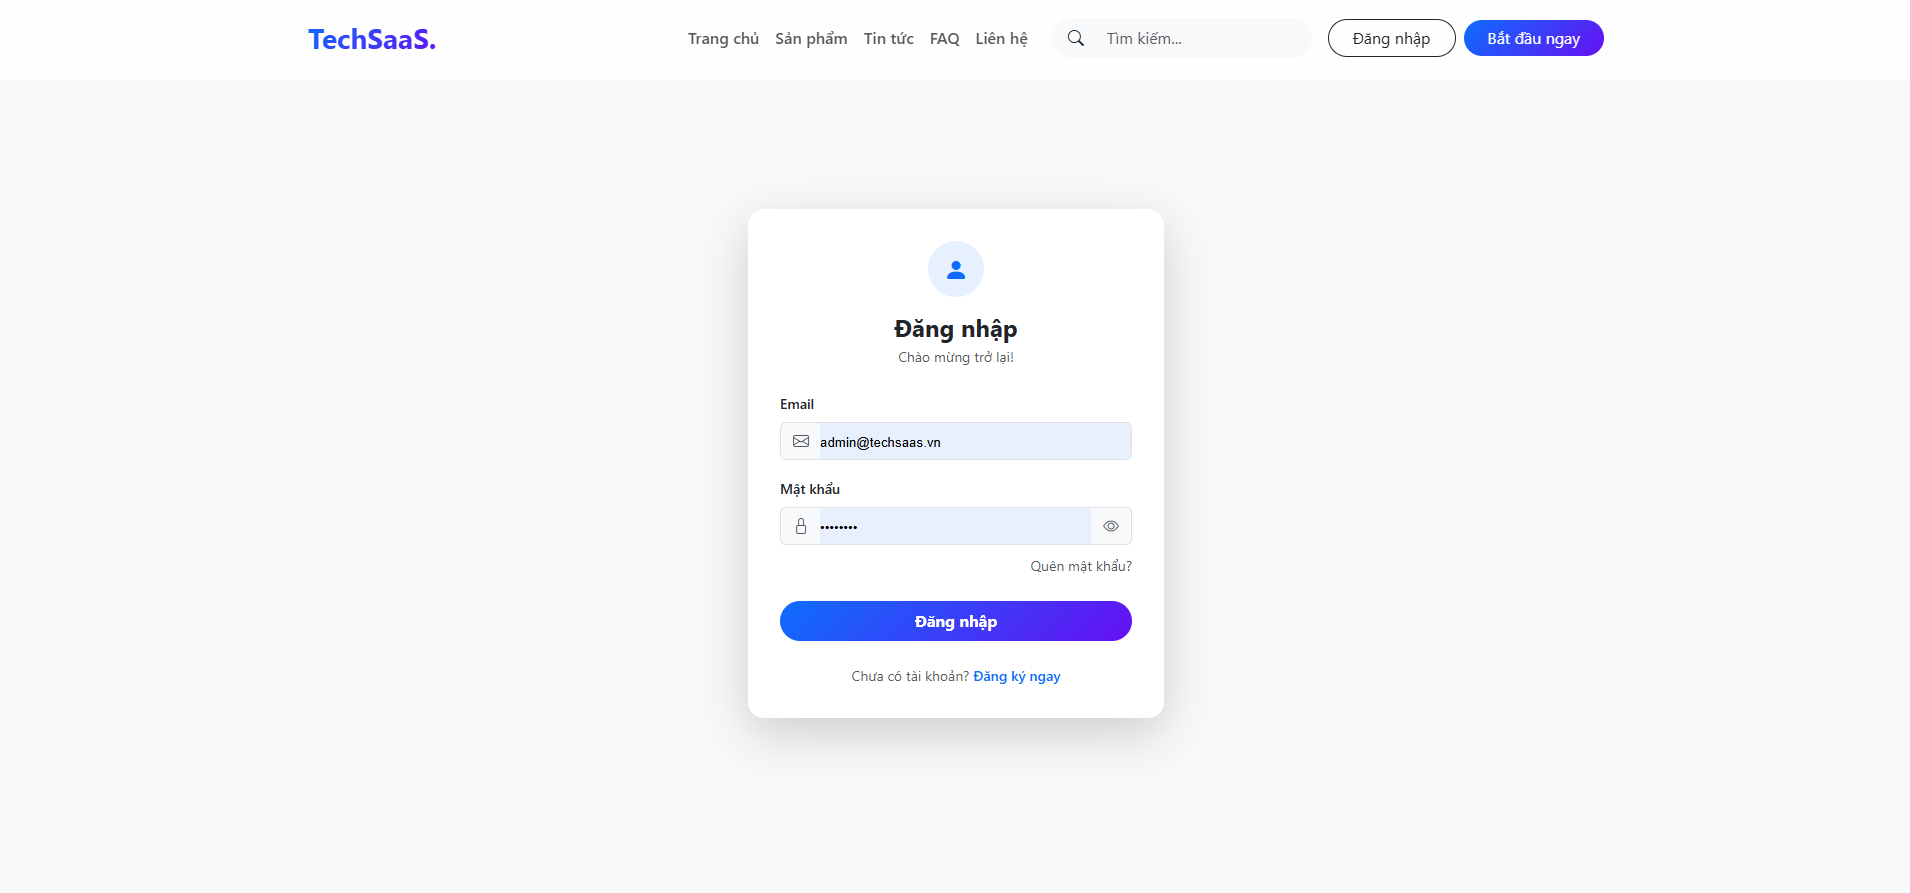
\includegraphics[width=\textwidth]{image/UI-Backend/Login.png}
        \caption*{Hệ thống đăng nhập Admin - Common Task}
    \end{minipage}
    \hfill
    \begin{minipage}{0.45\textwidth}
        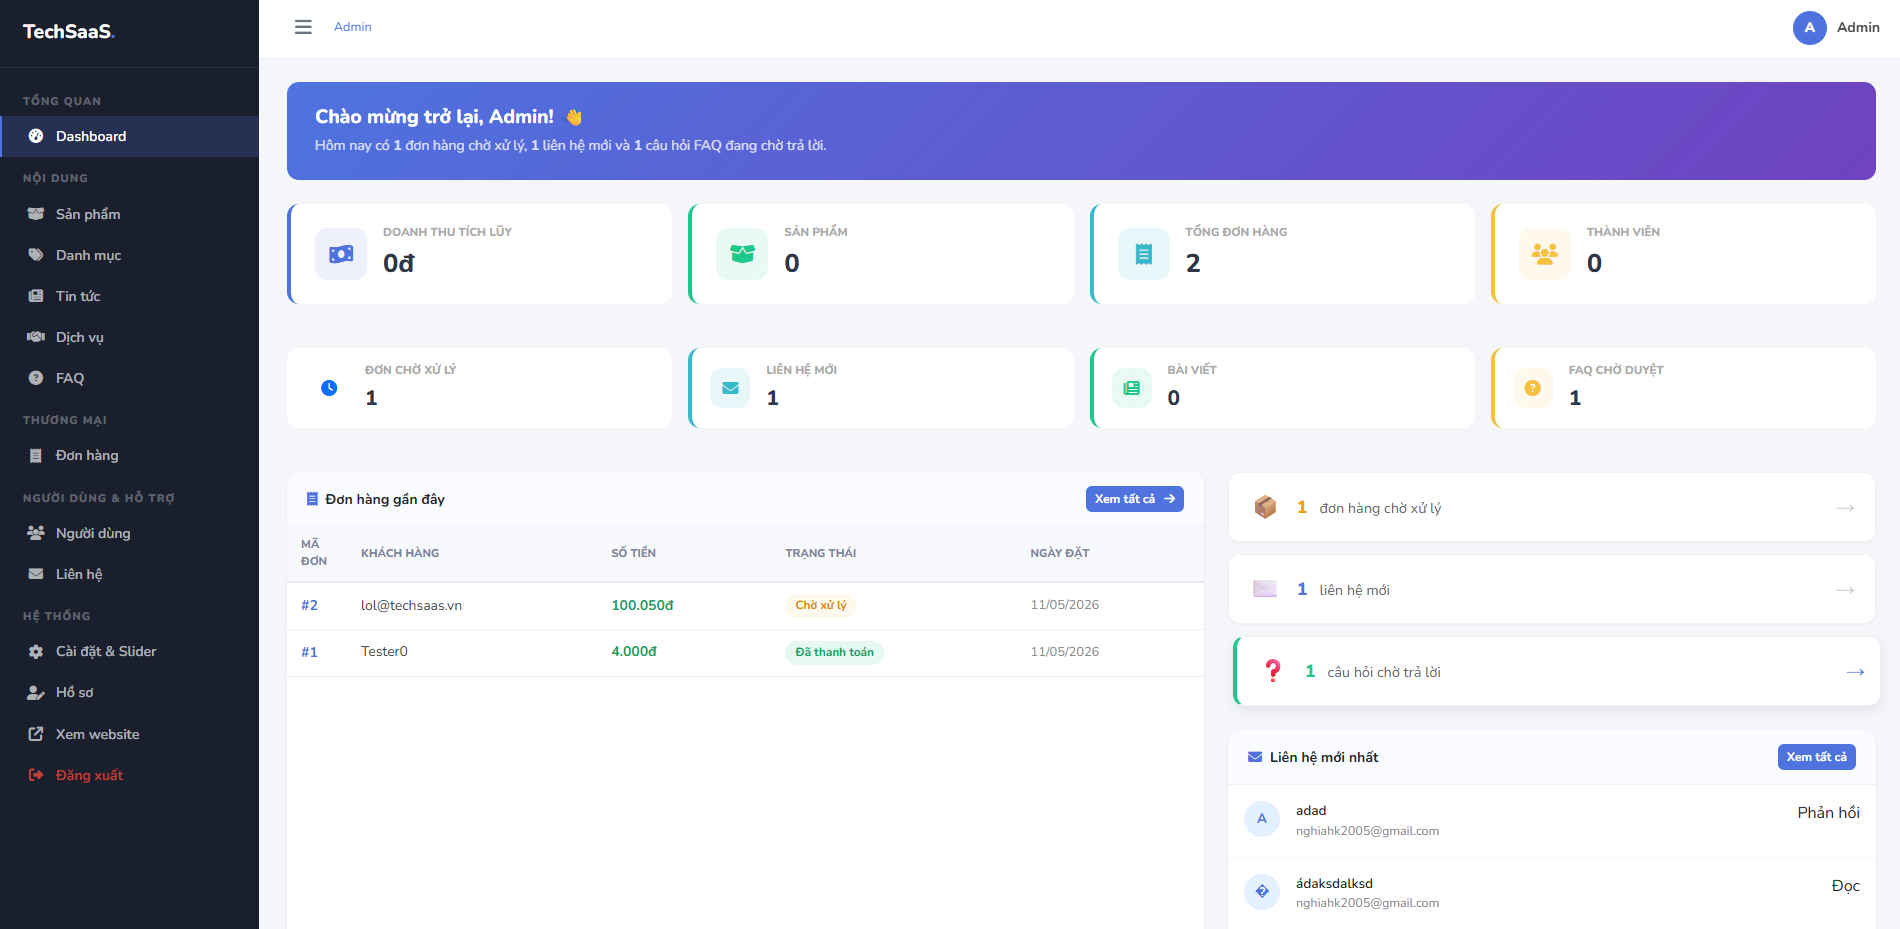
\includegraphics[width=\textwidth]{image/UI-Backend/Dashboard.png}
        \caption*{Bảng điều khiển thống kê tổng quát}
    \end{minipage}

    \vspace{0.5cm}

    \begin{minipage}{0.45\textwidth}
        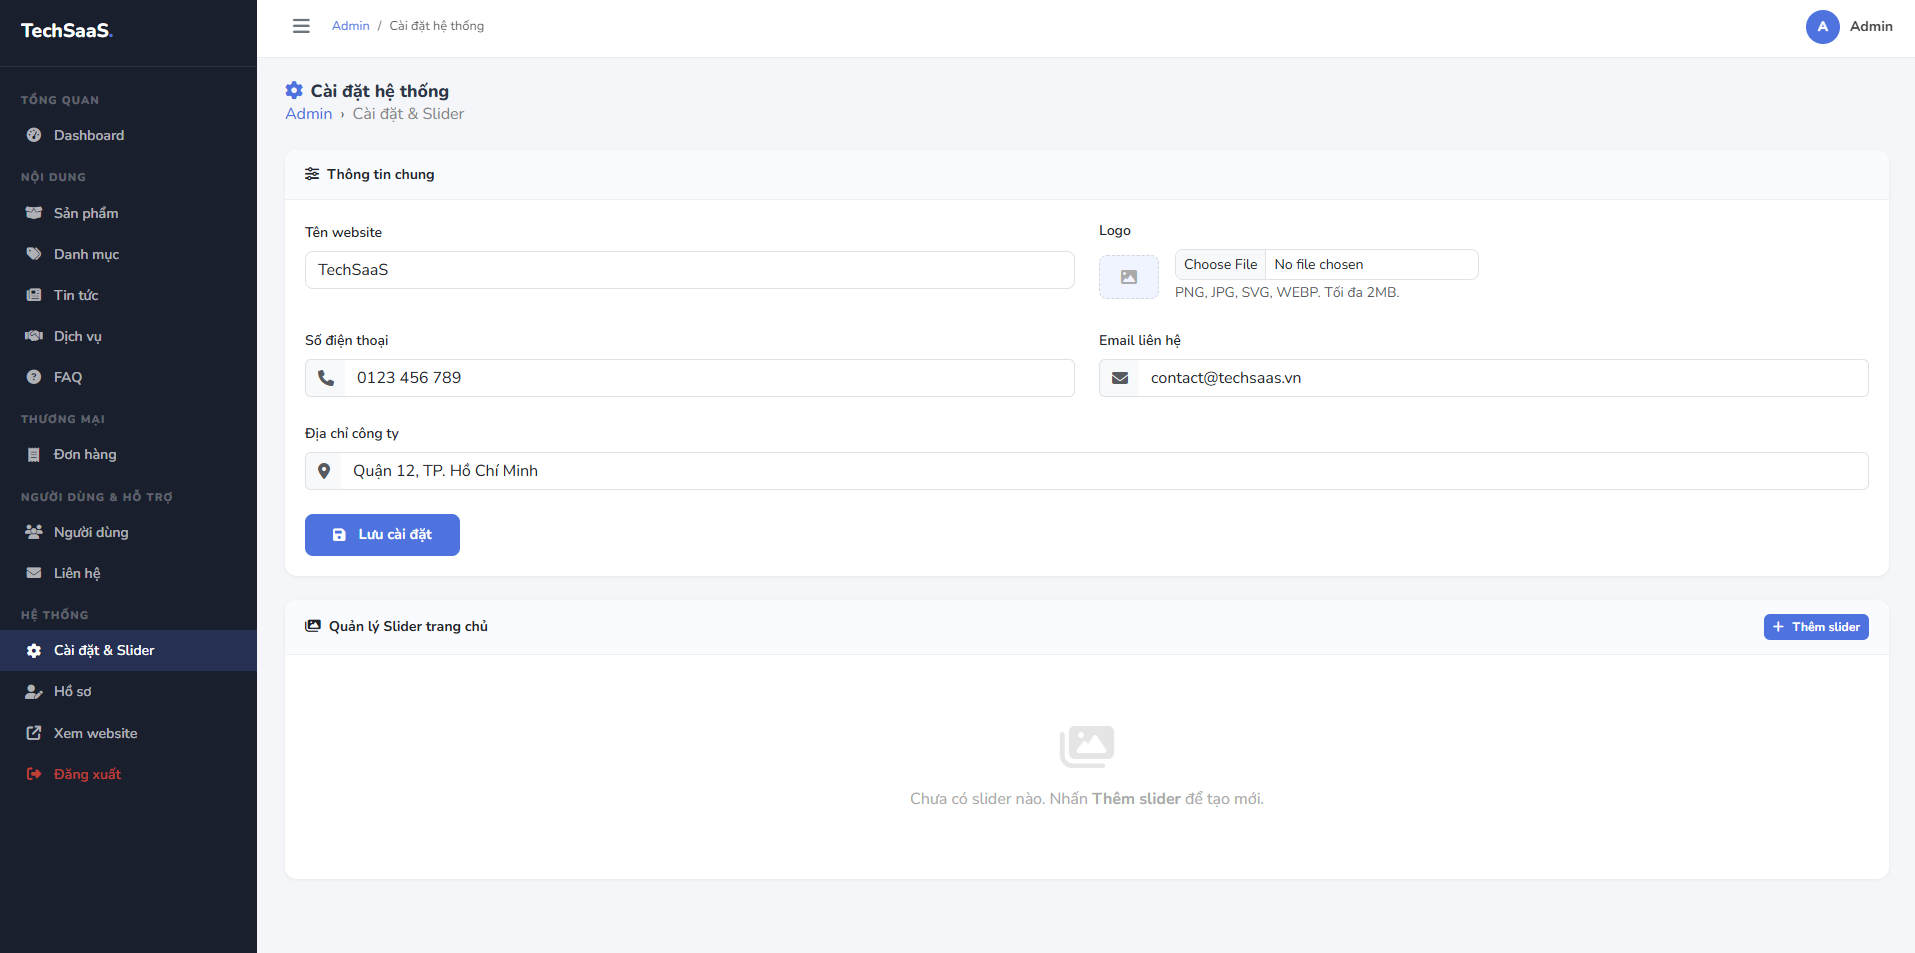
\includegraphics[width=\textwidth]{image/UI-Backend/Settings.png}
        \caption*{Cấu hình Hotline/Email - Task 1}
    \end{minipage}
    \hfill
    \begin{minipage}{0.45\textwidth}
        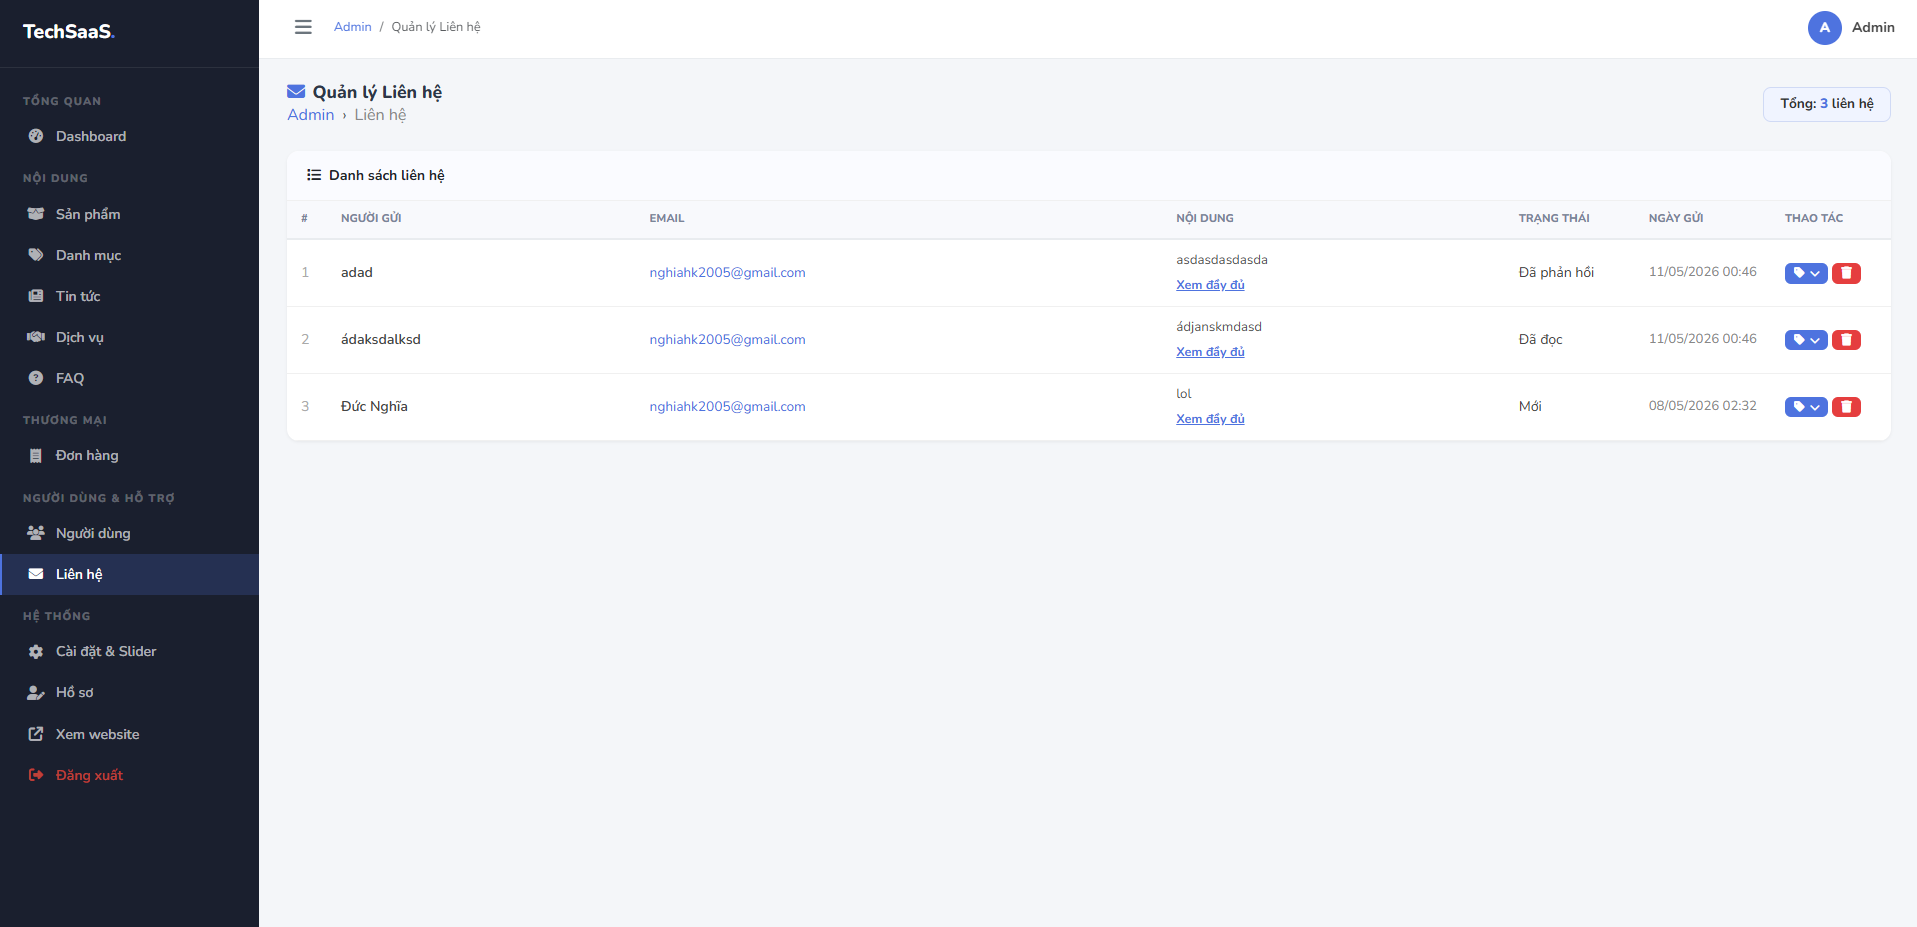
\includegraphics[width=\textwidth]{image/UI-Backend/Contact-List.png}
        \caption*{Quản lý danh sách liên hệ - Task 1}
    \end{minipage}
\end{figure}

\begin{figure}[H]
    \centering
    \begin{minipage}{0.45\textwidth}
        \includegraphics[width=\textwidth]{image/UI-Backend/About-Editor.png}
        \caption*{Biên tập nội dung Giới thiệu - Task 2}
    \end{minipage}
    \hfill
    \begin{minipage}{0.45\textwidth}
        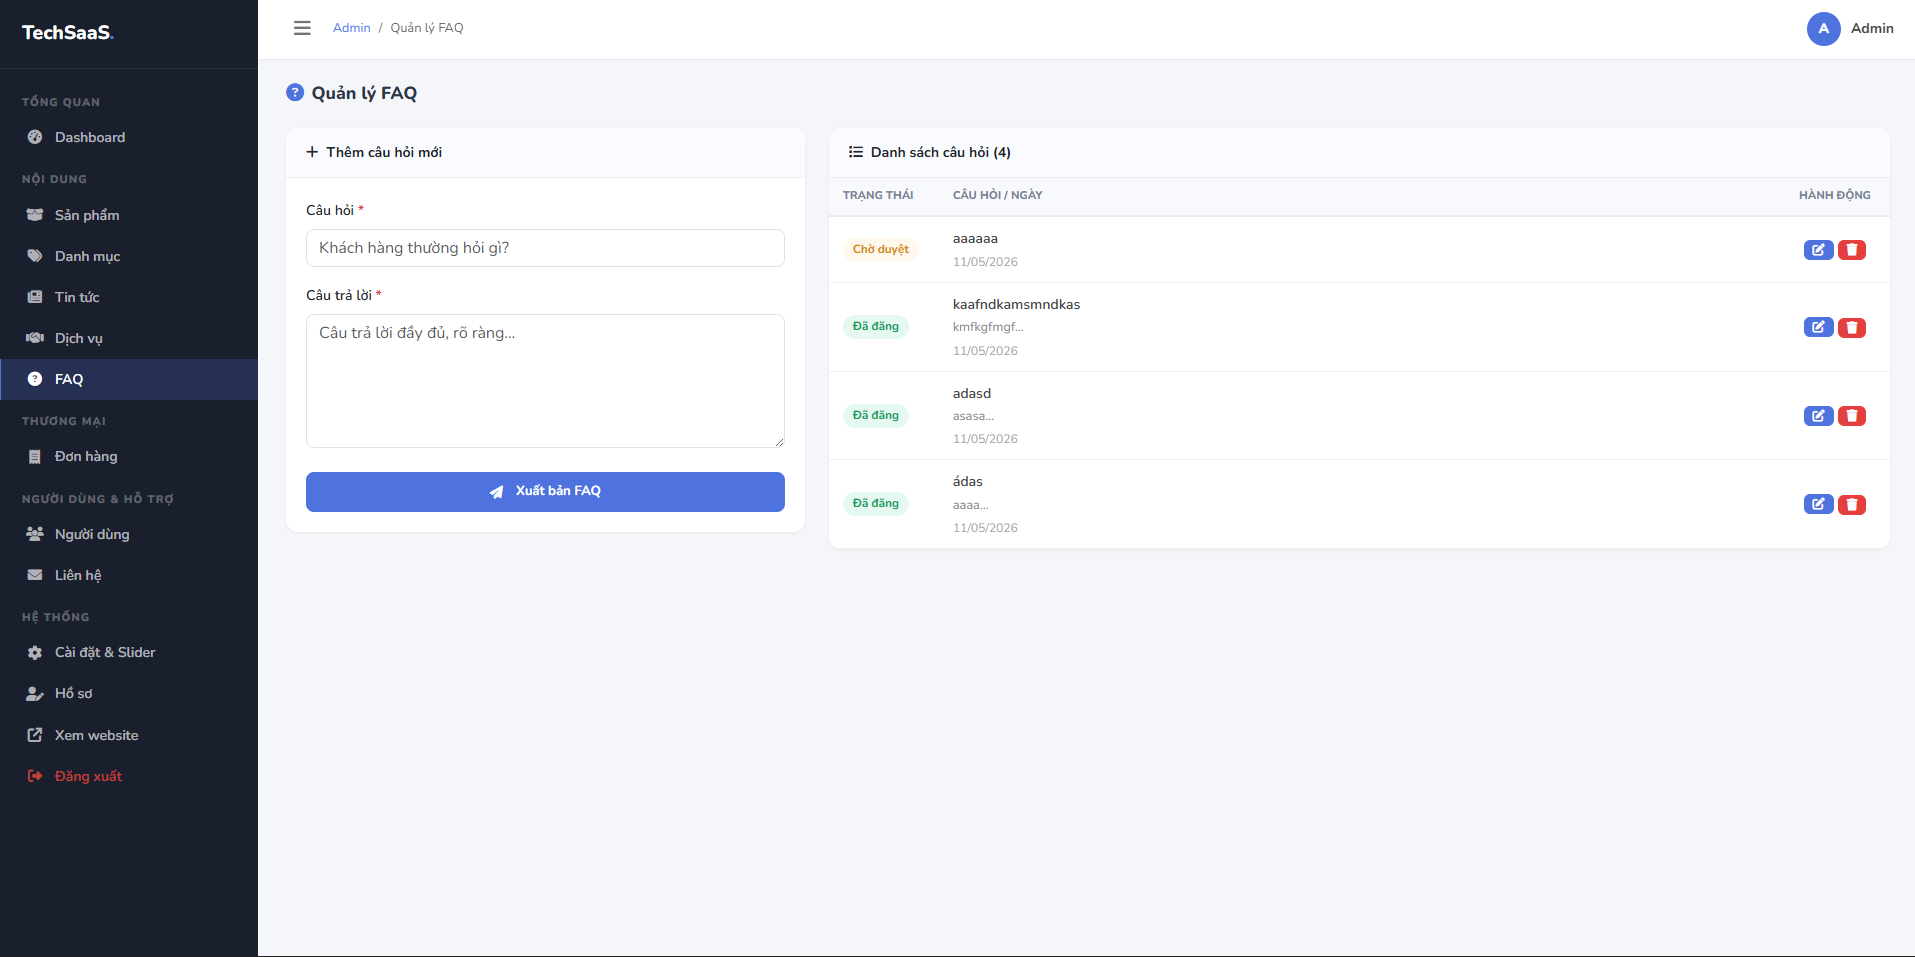
\includegraphics[width=\textwidth]{image/UI-Backend/QA-Manager.png}
        \caption*{Quản lý bộ câu hỏi Q\&A - Task 2}
    \end{minipage}

    \vspace{0.5cm}

    \begin{minipage}{0.45\textwidth}
        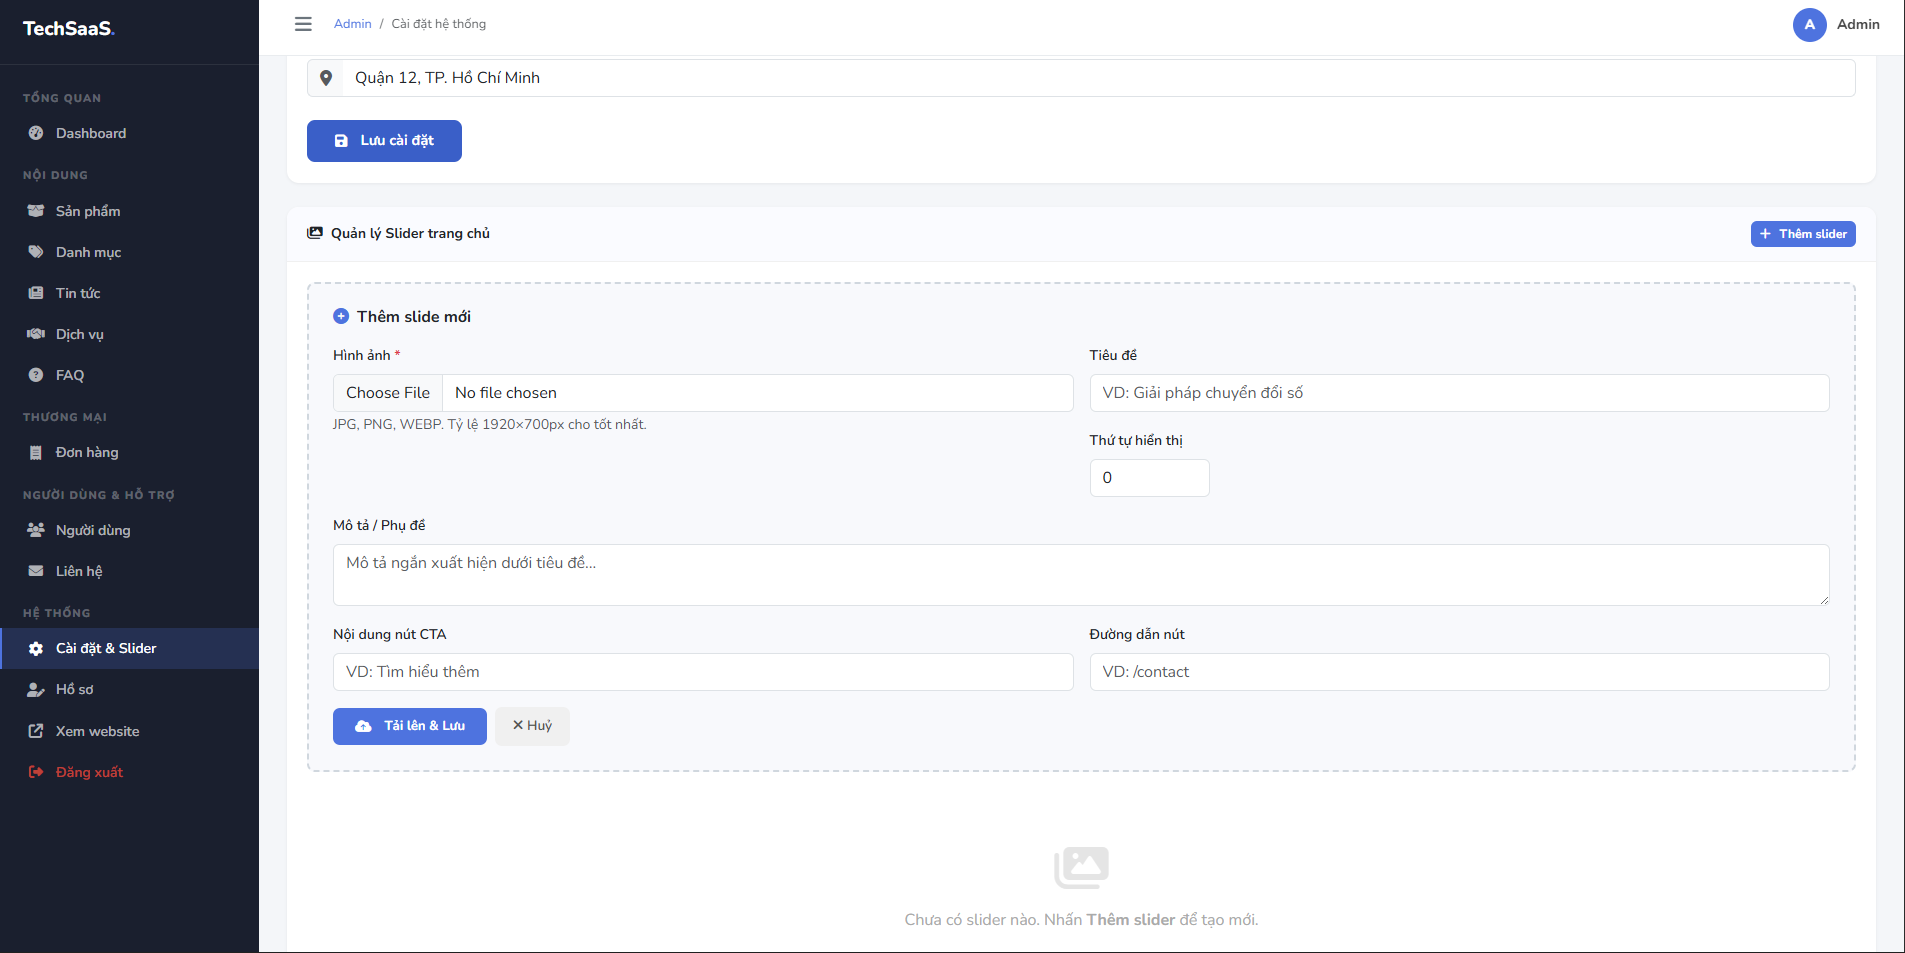
\includegraphics[width=\textwidth]{image/UI-Backend/Banner-Config.png}
        \caption*{Cập nhật hình ảnh Banner trang chủ}
    \end{minipage}
    \hfill
    \begin{minipage}{0.45\textwidth}
        \includegraphics[width=\textwidth]{image/UI-Backend/Logs.png}
        \caption*{Nhật ký hoạt động hệ thống}
    \end{minipage}
    \caption{Giao diện quản trị nội dung chuyên sâu phía Backend}
\end{figure}